\documentclass{beamer}
\usepackage[english]{babel}
\usepackage[utf8x]{inputenc}

\usepackage{xcolor}
\usepackage{graphicx}
\usepackage{color}
\usepackage{pifont}
\usepackage{url}
\usepackage{multimedia}
\usepackage[]{algorithm2e}
\usepackage{animate}
\usepackage{media9}
\usepackage{graphicx}
\usepackage[colorinlistoftodos]{todonotes}
\usepackage{ dsfont }
\usepackage{amsthm}
\usepackage{ stmaryrd }
\usepackage[]{algorithm2e}
\usepackage{amssymb}
\usepackage{mathrsfs}
\usepackage{float}

%\usetheme{AnnArbor}
%\usetheme{Antibes}
%\usetheme{Bergen}
%\usetheme{Berkeley}
%\usetheme{Berlin}
%\usetheme{Boadilla}
%\usetheme{boxes}
%\usetheme{CambridgeUS} %pourquoi pas
\usetheme{Copenhagen}  %pas mal
%\usetheme{Darmstadt}  %pas mal
%\usetheme{default}
%\usetheme{Frankfurt}
%\usetheme{Goettingen} %ça change
%\usetheme{Hannover} %même que goettingen pas à gauche
%\usetheme{Ilmenau}
%%%%\usetheme{JuanLesPins} %pas mal du tout
%\usetheme{Luebeck} % plus mastock
%\usetheme{Madrid}
%\usetheme{Malmoe}
%\usetheme{Marburg} %??
%\usetheme{Montpellier}
%\usetheme{PaloAlto}
%\usetheme{Pittsburgh}
%\usetheme{Rochester}
%\usetheme{Singapore}
%\usetheme{Szeged}
%\usetheme{Warsaw} %pas mal!


\begin{document}

    \title{ Numerical approximation of the Shallow Water model}

    % A subtitle is optional and this may be deleted
    \subtitle{}


    % - Give the names in the same order as the appear in the paper.
    % - Use the \inst{?} command only if the authors have different
    %   affiliation.
    \author{Mechineau Alexandre}

    \institute[University of Nantes]
    {M1 Mathematics \\University of Nantes \\
    Supervisor: Christophe Berthon}

    % - Use the \inst command only if there are several affiliations.
    % - Keep it simple, no one is interested in your street address.

    \date{2018, June}

    \begin{frame}
        \titlepage
    \end{frame}

    \section*{Introduction}

    \begin{frame}
        \frametitle{Introduction}
    \end{frame}
    
    
    \section*{Contents}
        \begin{frame}
                \tableofcontents
        \end{frame}
    
    \section{Analysis}
        \subsection{Linear Advection equation}
            \begin{frame}{Linear advection equation}
                Transport of a quantity by a constant speed fluid
                \begin{equation*}
                    \partial_t\varphi+ a\partial_x\varphi = 0, a \in \mathds{R}
                \end{equation*}
            \end{frame}
            \subsubsection{Characteristics curves}
                \begin{frame}{Characteristics curves}
                    \begin{equation*}
                        \partial_t\varphi+ a\partial_x\varphi = 0, a \in \mathds{R}
                    \end{equation*}
                    \pause
                    \begin{equation*}
                        X(t),~~ \dot X = a=\frac{dX}{dt}
                    \end{equation*}
                    \pause
                    We study $\varphi$ along the curve $X(t)$, then we have:
                    \begin{equation*}
                        \frac{d\varphi(X(t),t)}{dt}=0
                    \end{equation*}
                    \pause
                    The solution is so:
                    \begin{equation*}
                        \varphi(x,t) = \varphi_0(x-at)
                    \end{equation*}
                \end{frame}
                
                \begin{frame}{Characteristics curves : example}
                    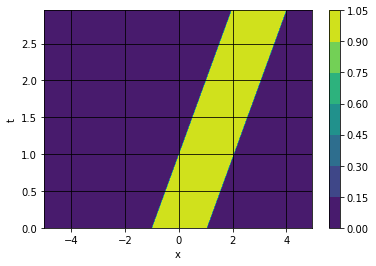
\includegraphics[width=10cm]{transport.png}
                \end{frame}
                
    
        \subsection{Burger's equation}
            \begin{frame}{Non-linear advection equation}
                \begin{equation*}
                    \partial_t u+ \partial_x f(u) = 0
                \end{equation*}
            \end{frame}
            \begin{frame}{Burger's equation}
                \begin{equation*}
                    \partial_t u+ \partial_x f(u) = 0, f(u)=\frac{u^2}{2}
                \end{equation*}
                It's the transport of a quantities where the speed of the fluid rely on the quantities 
                \begin{equation*}
                    \partial_t u+ u\partial_x u = 0
                \end{equation*}
            \end{frame}
            
            \begin{frame}{Characteristics curves}
                \begin{equation*}
                    {\dot X}\left(t\right) = f^\prime\left(u \left(X\left(t\right), t\right)\right)
                \end{equation*}
                \pause
                We have, like previously, that the solution is constant along the characteristics curves. Then, 
                \begin{equation*}
                    X\left(t\right) = f^\prime\left(u_0\left(x_0\right)\right)t + x_0
                \end{equation*}
            \end{frame}
            
            \begin{frame}{Discontinuity}
                Using $u(x,t=0) = sin(x) :$
                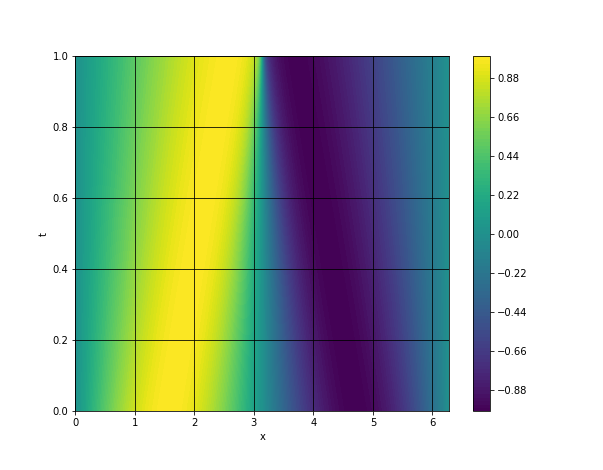
\includegraphics[width=8cm]{limit.png}
            \end{frame}
            
            \begin{frame}{Cauchy problem}
                Let f $\in \mathscr{C}^2, u_0 \in \mathscr{C}^1$ .\\
                Let T =  
                $
                \begin{cases}
                    +\infty\text{ if $x_0 \mapsto f^\prime\left(u_0\left(x_0\right)\right)$ is increasing}\\
                    - \frac{1}{\min \frac{d}{dx_0}f^\prime\left(u_0\left(x_0\right)\right)}\text{, else}
                \end{cases}
                $
           
                The following Cauchy problem :
                $
                \begin{cases}
                     d_t u + d_x f\left(u\right) = 0 \\
                    u\left(x,t=0\right) = u_0\left(x\right)
                    \end{cases}
                $
                admit a solution $u \in \mathscr{C}^1$ on $[0,T ]$.
            \end{frame}
            
            \begin{frame}{Lemma of  Rankine-Hugoniot}
                In a discontinuity, we have :
                \begin{equation*}
                    \sigma\left(u_R-u_L\right) + \left(f\left(u_R\right) - f\left(u_L\right)\right)=0
                \end{equation*}
                where $\sigma$ is the propagation speed of the discontinuity.
            \end{frame}
            
            \begin{frame}{Speed of the discontinuity}
                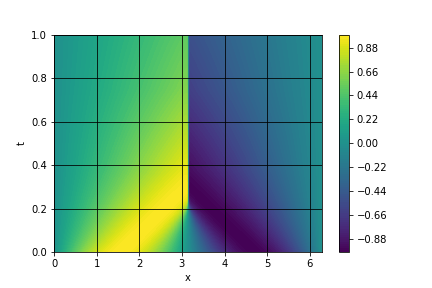
\includegraphics[width=8cm]{limtlt.png}
            \end{frame}
            
            \begin{frame}{Riemann problem}
                We want to solve : 
                    \begin{equation*}
                        d_t u + d_x f\left(u\right) = 0,\text{ f a {\bf convex} function}
                    \end{equation*}
                \pause
                With the following initial condition
                \begin{equation*}
                u\left(x,t=0\right) = 
                 \begin{cases}
                    u_L & \text{if $x < 0$}\\
                    u_R & \text{if $x \geq 0$}
                \end{cases}  
                \end{equation*}
            \end{frame}
            \begin{frame}{Solution of the Riemann problem}
                \begin{enumerate}
                    \uncover<1->{\item $u_L=u_R $, u is constant}
                    \uncover<2->{\item $u_L<u_R$, u is relaxation wave}
                    \uncover<3->{\item $u_L>u_R$, u is a shock wave}
                \end{enumerate}
            \end{frame}
            
            
            
    
        \subsection{Shallow water equation}
            \begin{frame}{Shallow water equation}
                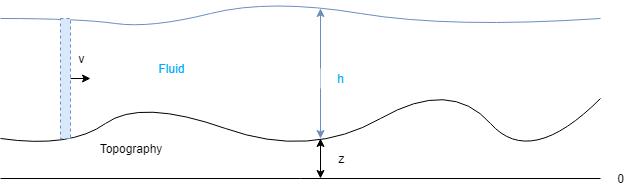
\includegraphics[width=12cm]{modele.png}
            \end{frame}
            \begin{frame}{Assumptions}
                \begin{enumerate}
                    \uncover<1->{\item The height of the fluid is smaller than the length of the domain}
                    \uncover<2->{\item The speed of the fluid is constant on a given column}
                \end{enumerate}
            \end{frame}
            \begin{frame}{Shallow water equation}
                \begin{align*}
                    &d_t h + d_x(hu) = 0 \\
                    &d_t(hu) + d_x\left( hu^2+ \frac{g}{2}gh^2 \right) = - hgz_x
                \end{align*}
            \end{frame}
            \begin{frame}{Shallow water equation}
                \begin{center}
                    Let U = $\begin{pmatrix} h \\ hu \end{pmatrix}$
                \end{center}
                
            \end{frame}
            \begin{frame}{Shallow water equation}
                \begin{center}
                    Let U = $\begin{pmatrix} h \\ hu \end{pmatrix}$ and $F(U)=\begin{pmatrix} hu \\ hu^2 + \frac{g}{2}h^2 \end{pmatrix}$
                \end{center}
                
            \end{frame}
            
            \begin{frame}{Shallow water equation}
                \begin{center}
                    Let U = $\begin{pmatrix} h \\ hu \end{pmatrix}$ and $F(U)=\begin{pmatrix} hu \\ hu^2 + \frac{g}{2}h^2 \end{pmatrix}$
                \end{center}
                
                \begin{align*}
                    &d_t h + d_x(hu) = 0 \\
                    &d_t(hu) + d_x\left( hu^2+ \frac{g}{2}gh^2 \right) = - hgz_x
                \end{align*}
            \end{frame}
            \begin{frame}{Shallow water equation}
                \begin{center}
                    Let U = $\begin{pmatrix} h \\ hu \end{pmatrix}$ and $F(U)=\begin{pmatrix} hu \\ hu^2 + \frac{g}{2}h^2 \end{pmatrix}$
                \end{center}
                
                \begin{align*}
                    &d_t U + d_x F(U) =  \begin{pmatrix}0\\ -hgz_x\end{pmatrix}\\
                \end{align*}
            \end{frame}
            
    \section{Numerical scheme}
        \subsection{Finite volume method}
            \begin{frame}{Finite volume method}
                \includegraphics[width=10cm]{Discretization.png}
            \end{frame}
        \subsection{Time discretization}
            \begin{frame}{Time discretization}
                Finite difference scheme:
                \begin{equation*}
                    \frac{du}{dt}\approx \frac{u_i^{t+1}-u_i^t}{\Delta t}
                \end{equation*}
            \end{frame}
            \begin{frame}{CFL condition}
                \textbf{Courant-Friedrichs-Lewy} condition : Best time step
                
            \end{frame}
        
        \subsection{Numerical Flux}
            \begin{frame}{Numerical Flux}\pause
                Flux exact: $F(U)$ \pause \\
                Numerical Flux : $\mathcal{F}_{i+\frac{1}{2}}(u_L, u_R)$ \pause \\
                Lax-Friedrichs scheme : $\mathcal{F}_{i+\frac{1}{2}}(u_L, u_R) =  \frac{1}{2}(F(u_L) + F(u_R)) - \frac{\Delta x}{2\Delta t}(u_R-u_L)$ 
                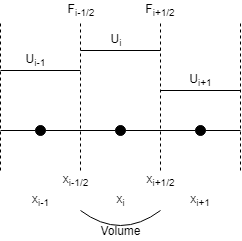
\includegraphics[width=5cm]{FluxBurger.png}
            \end{frame}
            \begin{frame}{Interpolation 1}
                \begin{center}
                    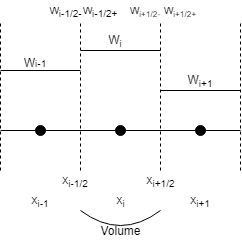
\includegraphics[width=6cm]{1storder.png}
                \end{center}
            \end{frame}
            
            \begin{frame}{Interpolation 2}
                \begin{center}
                    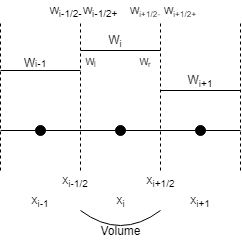
\includegraphics[width=6cm]{2ndorder.png}
                \end{center}
            \end{frame}
        
        %\subsection{Numerical scheme}
        %    \begin{frame}{Basic scheme}
        %        \begin{equation*}
        %                u^{t+1}_i=u^t_i - \frac{\Delta t}{\Delta x}(\mathcal{F}_{i+\frac{1}{2}} - \mathcal{F}_{i-\frac{1}{2}}),i\in\llbracket2,N-1\rrbracket
         %       \end{equation*}
        %    \end{frame}
            
        %    \begin{frame}{Well-balanced scheme 1st order, Shallow water equation}
        %        \begin{equation*}
        %            U_i^{t+1} = U_i^t - \frac{\Delta t}{\Delta x}(\mathcal{F}_{i+\frac{1}{2}} - \mathcal{F}_{i-\frac{1}{2}} - S_i),i\in\llbracket2,N-1\rrbracket
        %        \end{equation*}
        %    \end{frame}
            
        %    \begin{frame}{Well-balanced scheme 2nd order, Shallow water equation}
        %        \begin{equation*}
        %            U_i^{t+1} = U_i^t - \frac{\Delta t}{\Delta x}(\mathcal{F}_{i+\frac{1}{2}} - \mathcal{F}_{i-\frac{1}{2}} - S_i - S_{ci}),i\in\llbracket2,N-1\rrbracket
        %        \end{equation*}
        %    \end{frame}
    
    \section{Numerical results}
        \subsection{Burger's equation}
            \begin{frame}{Riemann problem: $u_L = u_R$}
                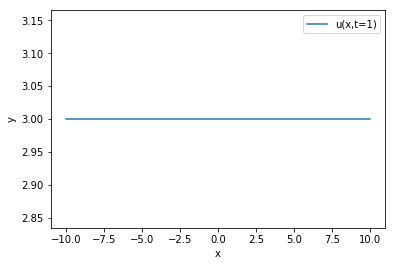
\includegraphics[width=9cm]{Burgers331.png}
            \end{frame}
            \begin{frame}{Riemann problem: $u_L < u_R$}
                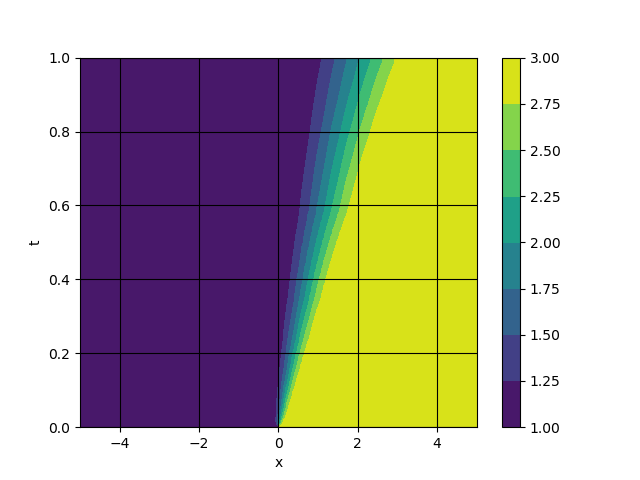
\includegraphics[width=9cm]{Burgers13.png}
            \end{frame}
            \begin{frame}{Riemann problem: $u_L > u_R$}
                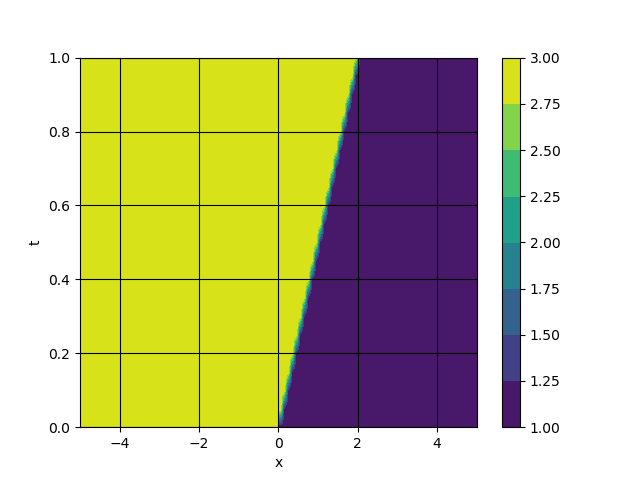
\includegraphics[width=9cm]{Burgers31.png}
            \end{frame}
        \subsection{Coupled equations}
            \begin{frame}{Dam burst}
                \pause
                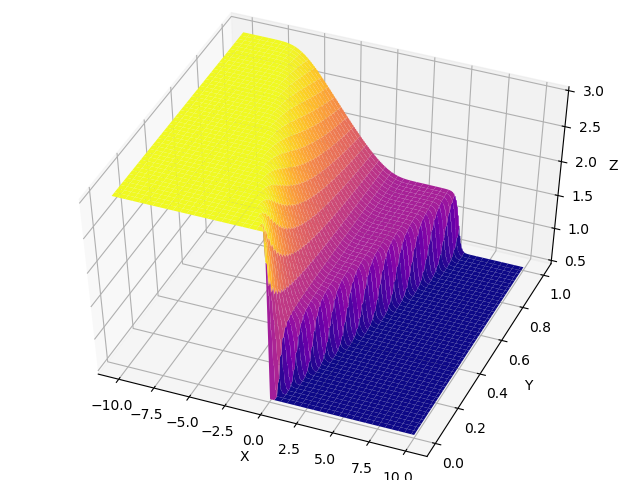
\includegraphics[width=8cm]{damLF0.png}
            \end{frame}
            \begin{frame}{Dam burst}
                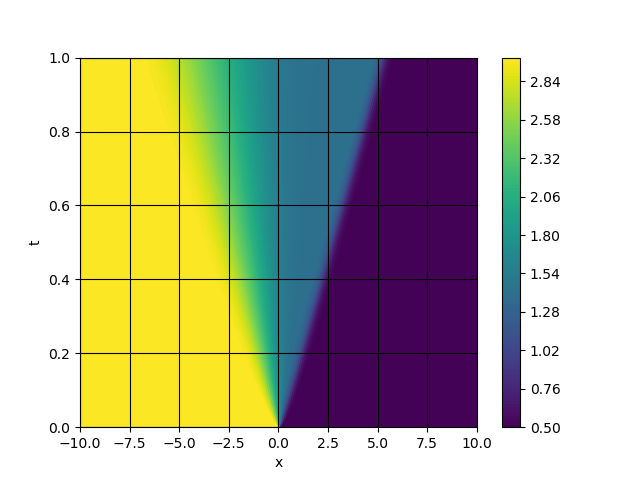
\includegraphics[width=8cm]{damLF0C.png}
            \end{frame}
        \subsection{Shallow water equation}
            \begin{frame}{Shallow water equation}
                \url{dam.mp4}
            \end{frame}
            
    \section{Conclusion}
        \begin{frame}{Conclusion}
            
        \end{frame}
        
        \subsection{Numerical scheme}
        \begin{frame}{Numerical flux, finite difference }
            \begin{enumerate}
            \uncover<1->{\item Increase the order of the time finite difference}
            \uncover<2->{\item Use a better numerical flux }
        \end{enumerate}
        \end{frame}
        
        \subsection{Implementation}
        \begin{frame}{Parallel computing}
        \begin{enumerate}
            \uncover<1->{\item Easy to split a step in several simple tasks }
            \uncover<2->{\item Low data dependency}
        \end{enumerate}
            
        \end{frame}
  
\end{document}